% Options for packages loaded elsewhere
\PassOptionsToPackage{unicode}{hyperref}
\PassOptionsToPackage{hyphens}{url}
%
\documentclass[
]{book}
\usepackage{amsmath,amssymb}
\usepackage{iftex}
\ifPDFTeX
  \usepackage[T1]{fontenc}
  \usepackage[utf8]{inputenc}
  \usepackage{textcomp} % provide euro and other symbols
\else % if luatex or xetex
  \usepackage{unicode-math} % this also loads fontspec
  \defaultfontfeatures{Scale=MatchLowercase}
  \defaultfontfeatures[\rmfamily]{Ligatures=TeX,Scale=1}
\fi
\usepackage{lmodern}
\ifPDFTeX\else
  % xetex/luatex font selection
\fi
% Use upquote if available, for straight quotes in verbatim environments
\IfFileExists{upquote.sty}{\usepackage{upquote}}{}
\IfFileExists{microtype.sty}{% use microtype if available
  \usepackage[]{microtype}
  \UseMicrotypeSet[protrusion]{basicmath} % disable protrusion for tt fonts
}{}
\makeatletter
\@ifundefined{KOMAClassName}{% if non-KOMA class
  \IfFileExists{parskip.sty}{%
    \usepackage{parskip}
  }{% else
    \setlength{\parindent}{0pt}
    \setlength{\parskip}{6pt plus 2pt minus 1pt}}
}{% if KOMA class
  \KOMAoptions{parskip=half}}
\makeatother
\usepackage{xcolor}
\usepackage{color}
\usepackage{fancyvrb}
\newcommand{\VerbBar}{|}
\newcommand{\VERB}{\Verb[commandchars=\\\{\}]}
\DefineVerbatimEnvironment{Highlighting}{Verbatim}{commandchars=\\\{\}}
% Add ',fontsize=\small' for more characters per line
\usepackage{framed}
\definecolor{shadecolor}{RGB}{248,248,248}
\newenvironment{Shaded}{\begin{snugshade}}{\end{snugshade}}
\newcommand{\AlertTok}[1]{\textcolor[rgb]{0.94,0.16,0.16}{#1}}
\newcommand{\AnnotationTok}[1]{\textcolor[rgb]{0.56,0.35,0.01}{\textbf{\textit{#1}}}}
\newcommand{\AttributeTok}[1]{\textcolor[rgb]{0.13,0.29,0.53}{#1}}
\newcommand{\BaseNTok}[1]{\textcolor[rgb]{0.00,0.00,0.81}{#1}}
\newcommand{\BuiltInTok}[1]{#1}
\newcommand{\CharTok}[1]{\textcolor[rgb]{0.31,0.60,0.02}{#1}}
\newcommand{\CommentTok}[1]{\textcolor[rgb]{0.56,0.35,0.01}{\textit{#1}}}
\newcommand{\CommentVarTok}[1]{\textcolor[rgb]{0.56,0.35,0.01}{\textbf{\textit{#1}}}}
\newcommand{\ConstantTok}[1]{\textcolor[rgb]{0.56,0.35,0.01}{#1}}
\newcommand{\ControlFlowTok}[1]{\textcolor[rgb]{0.13,0.29,0.53}{\textbf{#1}}}
\newcommand{\DataTypeTok}[1]{\textcolor[rgb]{0.13,0.29,0.53}{#1}}
\newcommand{\DecValTok}[1]{\textcolor[rgb]{0.00,0.00,0.81}{#1}}
\newcommand{\DocumentationTok}[1]{\textcolor[rgb]{0.56,0.35,0.01}{\textbf{\textit{#1}}}}
\newcommand{\ErrorTok}[1]{\textcolor[rgb]{0.64,0.00,0.00}{\textbf{#1}}}
\newcommand{\ExtensionTok}[1]{#1}
\newcommand{\FloatTok}[1]{\textcolor[rgb]{0.00,0.00,0.81}{#1}}
\newcommand{\FunctionTok}[1]{\textcolor[rgb]{0.13,0.29,0.53}{\textbf{#1}}}
\newcommand{\ImportTok}[1]{#1}
\newcommand{\InformationTok}[1]{\textcolor[rgb]{0.56,0.35,0.01}{\textbf{\textit{#1}}}}
\newcommand{\KeywordTok}[1]{\textcolor[rgb]{0.13,0.29,0.53}{\textbf{#1}}}
\newcommand{\NormalTok}[1]{#1}
\newcommand{\OperatorTok}[1]{\textcolor[rgb]{0.81,0.36,0.00}{\textbf{#1}}}
\newcommand{\OtherTok}[1]{\textcolor[rgb]{0.56,0.35,0.01}{#1}}
\newcommand{\PreprocessorTok}[1]{\textcolor[rgb]{0.56,0.35,0.01}{\textit{#1}}}
\newcommand{\RegionMarkerTok}[1]{#1}
\newcommand{\SpecialCharTok}[1]{\textcolor[rgb]{0.81,0.36,0.00}{\textbf{#1}}}
\newcommand{\SpecialStringTok}[1]{\textcolor[rgb]{0.31,0.60,0.02}{#1}}
\newcommand{\StringTok}[1]{\textcolor[rgb]{0.31,0.60,0.02}{#1}}
\newcommand{\VariableTok}[1]{\textcolor[rgb]{0.00,0.00,0.00}{#1}}
\newcommand{\VerbatimStringTok}[1]{\textcolor[rgb]{0.31,0.60,0.02}{#1}}
\newcommand{\WarningTok}[1]{\textcolor[rgb]{0.56,0.35,0.01}{\textbf{\textit{#1}}}}
\usepackage{longtable,booktabs,array}
\usepackage{calc} % for calculating minipage widths
% Correct order of tables after \paragraph or \subparagraph
\usepackage{etoolbox}
\makeatletter
\patchcmd\longtable{\par}{\if@noskipsec\mbox{}\fi\par}{}{}
\makeatother
% Allow footnotes in longtable head/foot
\IfFileExists{footnotehyper.sty}{\usepackage{footnotehyper}}{\usepackage{footnote}}
\makesavenoteenv{longtable}
\usepackage{graphicx}
\makeatletter
\def\maxwidth{\ifdim\Gin@nat@width>\linewidth\linewidth\else\Gin@nat@width\fi}
\def\maxheight{\ifdim\Gin@nat@height>\textheight\textheight\else\Gin@nat@height\fi}
\makeatother
% Scale images if necessary, so that they will not overflow the page
% margins by default, and it is still possible to overwrite the defaults
% using explicit options in \includegraphics[width, height, ...]{}
\setkeys{Gin}{width=\maxwidth,height=\maxheight,keepaspectratio}
% Set default figure placement to htbp
\makeatletter
\def\fps@figure{htbp}
\makeatother
\setlength{\emergencystretch}{3em} % prevent overfull lines
\providecommand{\tightlist}{%
  \setlength{\itemsep}{0pt}\setlength{\parskip}{0pt}}
\setcounter{secnumdepth}{5}
\usepackage{booktabs}
\usepackage{amsthm}
\makeatletter
\def\thm@space@setup{%
  \thm@preskip=8pt plus 2pt minus 4pt
  \thm@postskip=\thm@preskip
}
\makeatother
\ifLuaTeX
  \usepackage{selnolig}  % disable illegal ligatures
\fi
\usepackage[]{natbib}
\bibliographystyle{apalike}
\IfFileExists{bookmark.sty}{\usepackage{bookmark}}{\usepackage{hyperref}}
\IfFileExists{xurl.sty}{\usepackage{xurl}}{} % add URL line breaks if available
\urlstyle{same}
\hypersetup{
  pdftitle={Business Mathematics},
  pdfauthor={Siju Swamy},
  hidelinks,
  pdfcreator={LaTeX via pandoc}}

\title{Business Mathematics}
\author{Siju Swamy}
\date{2023-08-27}

\usepackage{amsthm}
\newtheorem{theorem}{Theorem}[chapter]
\newtheorem{lemma}{Lemma}[chapter]
\newtheorem{corollary}{Corollary}[chapter]
\newtheorem{proposition}{Proposition}[chapter]
\newtheorem{conjecture}{Conjecture}[chapter]
\theoremstyle{definition}
\newtheorem{definition}{Definition}[chapter]
\theoremstyle{definition}
\newtheorem{example}{Example}[chapter]
\theoremstyle{definition}
\newtheorem{exercise}{Exercise}[chapter]
\theoremstyle{definition}
\newtheorem{hypothesis}{Hypothesis}[chapter]
\theoremstyle{remark}
\newtheorem*{remark}{Remark}
\newtheorem*{solution}{Solution}
\begin{document}
\maketitle

{
\setcounter{tocdepth}{1}
\tableofcontents
}
\hypertarget{prerequisites}{%
\chapter{Prerequisites}\label{prerequisites}}

To study this course, a basic understanding of Class 10 mathematics is sufficient.

\begin{Shaded}
\begin{Highlighting}[]
\FunctionTok{install.packages}\NormalTok{(}\StringTok{"bookdown"}\NormalTok{)}
\CommentTok{\# or the development version}
\CommentTok{\# devtools::install\_github("rstudio/bookdown")}
\end{Highlighting}
\end{Shaded}

\hypertarget{intro}{%
\chapter{Introduction}\label{intro}}

\hypertarget{introduction-to-business-mathematics-for-mba-students}{%
\section{Introduction to Business Mathematics for MBA Students}\label{introduction-to-business-mathematics-for-mba-students}}

Welcome to the world of Business Mathematics! In the dynamic landscape of modern business, mathematical tools and techniques play a crucial role in decision-making, strategic planning, financial analysis, and overall management. This course is designed to equip MBA students like you with the foundational knowledge and skills needed to navigate the complex mathematical aspects of the business world.

\hypertarget{course-objectives}{%
\subsection{Course Objectives:}\label{course-objectives}}

The primary objective of this course is to provide you with a solid foundation in various mathematical concepts and their practical applications in the business context. By the end of this course, you should be able to:

\begin{quote}
Quantitative Analysis: Apply mathematical tools to analyze quantitative data, allowing you to make informed business decisions based on numerical insights.
\end{quote}

\begin{quote}
Financial Analysis: Understand and interpret financial data, perform financial calculations, and assess the financial health of organizations.
\end{quote}

\begin{quote}
Optimization: Utilize mathematical techniques to optimize resource allocation, production processes, inventory management, and more, in order to enhance operational efficiency.
\end{quote}

\begin{quote}
Time Value of Money: Grasp the fundamental concept of time value of money, including present and future value calculations, and their significance in financial decision-making.
\end{quote}

\begin{quote}
Business Forecasting: Acquire skills to predict future trends and make informed projections by using mathematical models and statistical techniques.
\end{quote}

\begin{quote}
Decision Making: Develop the ability to solve complex business problems using quantitative methods, aiding in effective decision-making and strategic planning.
\end{quote}

\hypertarget{teaching-methodology}{%
\section{Teaching Methodology:}\label{teaching-methodology}}

Throughout the course, a combination of lectures, real-world case studies, hands-on exercises, and interactive discussions will be employed to help you grasp both the theoretical concepts and practical applications of business mathematics. Collaborative learning and critical thinking will be encouraged, as you work individually and in groups to solve complex business problems.

Remember, the knowledge gained from this course will serve as a valuable toolset in your MBA journey and beyond. So, let's embark on this mathematical exploration together, and discover how numbers can drive informed decisions and foster success in the world of business!

You can label chapter and section titles using \texttt{\{\#label\}} after them, e.g., we can reference Chapter \ref{intro}. If you do not manually label them, there will be automatic labels anyway, e.g., Chapter \ref{methods}.

Figures and tables with captions will be placed in \texttt{figure} and \texttt{table} environments, respectively.

\begin{Shaded}
\begin{Highlighting}[]
\FunctionTok{par}\NormalTok{(}\AttributeTok{mar =} \FunctionTok{c}\NormalTok{(}\DecValTok{4}\NormalTok{, }\DecValTok{4}\NormalTok{, .}\DecValTok{1}\NormalTok{, .}\DecValTok{1}\NormalTok{))}
\FunctionTok{plot}\NormalTok{(pressure, }\AttributeTok{type =} \StringTok{\textquotesingle{}b\textquotesingle{}}\NormalTok{, }\AttributeTok{pch =} \DecValTok{19}\NormalTok{)}
\end{Highlighting}
\end{Shaded}

\begin{figure}

{\centering 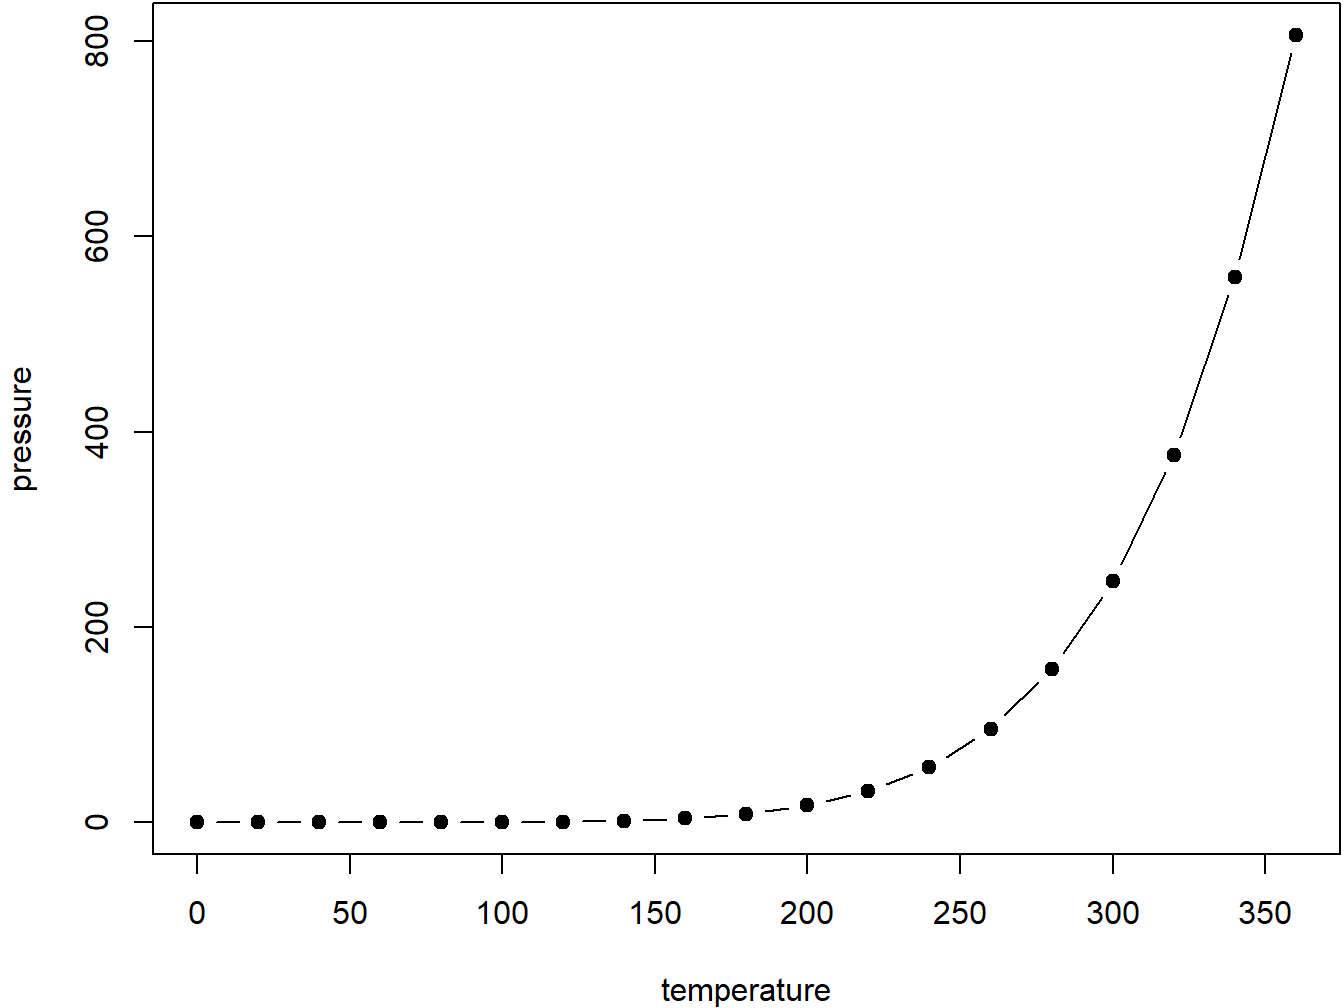
\includegraphics[width=0.8\linewidth]{bookdown-demo_files/figure-latex/nice-fig-1} 

}

\caption{Here is a nice figure!}\label{fig:nice-fig}
\end{figure}

Reference a figure by its code chunk label with the \texttt{fig:} prefix, e.g., see Figure \ref{fig:nice-fig}. Similarly, you can reference tables generated from \texttt{knitr::kable()}, e.g., see Table \ref{tab:nice-tab}.

\begin{Shaded}
\begin{Highlighting}[]
\NormalTok{knitr}\SpecialCharTok{::}\FunctionTok{kable}\NormalTok{(}
  \FunctionTok{head}\NormalTok{(iris, }\DecValTok{20}\NormalTok{), }\AttributeTok{caption =} \StringTok{\textquotesingle{}Here is a nice table!\textquotesingle{}}\NormalTok{,}
  \AttributeTok{booktabs =} \ConstantTok{TRUE}
\NormalTok{)}
\end{Highlighting}
\end{Shaded}

\begin{table}

\caption{\label{tab:nice-tab}Here is a nice table!}
\centering
\begin{tabular}[t]{rrrrl}
\toprule
Sepal.Length & Sepal.Width & Petal.Length & Petal.Width & Species\\
\midrule
5.1 & 3.5 & 1.4 & 0.2 & setosa\\
4.9 & 3.0 & 1.4 & 0.2 & setosa\\
4.7 & 3.2 & 1.3 & 0.2 & setosa\\
4.6 & 3.1 & 1.5 & 0.2 & setosa\\
5.0 & 3.6 & 1.4 & 0.2 & setosa\\
\addlinespace
5.4 & 3.9 & 1.7 & 0.4 & setosa\\
4.6 & 3.4 & 1.4 & 0.3 & setosa\\
5.0 & 3.4 & 1.5 & 0.2 & setosa\\
4.4 & 2.9 & 1.4 & 0.2 & setosa\\
4.9 & 3.1 & 1.5 & 0.1 & setosa\\
\addlinespace
5.4 & 3.7 & 1.5 & 0.2 & setosa\\
4.8 & 3.4 & 1.6 & 0.2 & setosa\\
4.8 & 3.0 & 1.4 & 0.1 & setosa\\
4.3 & 3.0 & 1.1 & 0.1 & setosa\\
5.8 & 4.0 & 1.2 & 0.2 & setosa\\
\addlinespace
5.7 & 4.4 & 1.5 & 0.4 & setosa\\
5.4 & 3.9 & 1.3 & 0.4 & setosa\\
5.1 & 3.5 & 1.4 & 0.3 & setosa\\
5.7 & 3.8 & 1.7 & 0.3 & setosa\\
5.1 & 3.8 & 1.5 & 0.3 & setosa\\
\bottomrule
\end{tabular}
\end{table}

You can write citations, too. For example, we are using the \textbf{bookdown} package \citep{R-bookdown} in this sample book, which was built on top of R Markdown and \textbf{knitr} \citep{xie2015}.

\hypertarget{set-theory-operations}{%
\chapter{Set Theory \& Operations}\label{set-theory-operations}}

\begin{center}\rule{0.5\linewidth}{0.5pt}\end{center}

Set theory \& Operations: Introduction, Definition, elements and types of sets, operations on sets, De-Morgan's Law and Cartesian product of two sets. Definition of a vector, Types of Vectors, Addition and subtraction of vectors, Multiplication of a vector by a scalar, Product of two vectors.

\begin{center}\rule{0.5\linewidth}{0.5pt}\end{center}

\hypertarget{introduction-of-set-theory}{%
\section{Introduction of set theory}\label{introduction-of-set-theory}}

Set theory, branch of mathematics that deals with the properties of well-defined collections of objects, which may or may not be of a mathematical nature, such as numbers or functions. The theory is less valuable in direct application to ordinary experience than as a basis for precise and adaptable terminology for the definition of complex and sophisticated mathematical concepts.

Between the years 1874 and 1897, the German mathematician and logician Georg Cantor created a theory of abstract sets of entities and made it into a mathematical discipline. This theory grew out of his investigations of some concrete problems regarding certain types of infinite sets of real numbers. A set, wrote Cantor, is a collection of definite, distinguishable objects of perception or thought conceived as a whole. The objects are called elements or members of the set.

The theory had the revolutionary aspect of treating infinite sets as mathematical objects that are on an equal footing with those that can be constructed in a finite number of steps. Since antiquity, a majority of mathematicians had carefully avoided the introduction into their arguments of the actual infinite (i.e., of sets containing an infinity of objects conceived as existing simultaneously, at least in thought). Since this attitude persisted until almost the end of the 19th century, Cantor's work was the subject of much criticism to the effect that it dealt with fictions---indeed, that it encroached on the domain of philosophers and violated the principles of religion. Once applications to analysis began to be found, however, attitudes began to change, and by the 1890s Cantor's ideas and results were gaining acceptance. By 1900, set theory was recognized as a distinct branch of mathematics.

At just that time, however, several contradictions in so-called naive set theory were discovered. In order to eliminate such problems, an axiomatic basis was developed for the theory of sets analogous to that developed for elementary geometry. The degree of success that has been achieved in this development, as well as the present stature of set theory, has been well expressed in the Nicolas Bourbaki Éléments de mathématique (begun 1939; ``Elements of Mathematics''): ``Nowadays it is known to be possible, logically speaking, to derive practically the whole of known mathematics from a single source, The Theory of Sets.''

\hypertarget{definitions}{%
\section{Definitions}\label{definitions}}

\begin{definition}[Set]
\protect\hypertarget{def:set}{}\label{def:set}A set is a well defined collection or class of objects
\end{definition}

Sets can be related to many real-life examples, such as the number of rivers in India, number of colours in a rainbow, etc.The following are the simple examples of sets as per definition \ref{def:set}.

\begin{enumerate}
\def\labelenumi{\arabic{enumi}.}
\item
  The numbers 1,2,3.
\item
  The planets in the universe.
\item
  The vowels in english alphabets.
\item
  The set of all students in the IMBA class.
\item
  The set of countries in the world.
\end{enumerate}

\begin{example}[Practical example]
\protect\hypertarget{exm:ex1}{}\label{exm:ex1}To understand sets, consider a practical scenario. While going to school from home, Nivy decided to note down the names of restaurants which come in between. The list of the restaurants, in the order they came, was:

\[ \begin{array}{l} List\ 1: R_A ~~~~~       R_B ~~~~~       R_C ~~~~~       R_D ~~~~~       R_E \end{array}\]

The above-mentioned list is a collection of objects. Also, it is well-defined. By well-defined, it is meant that anyone should be able to tell whether the object belongs to the particular collection or not. E. g. a stationary shop can't come in the category of the restaurants. If the collection of objects is well-defined, it is known as a set.

The objects in a set are referred to as \emph{elements of the set}. A set can have finite or infinite elements. While coming back from the school, Nivy wanted to confirm the list what she had made earlier. This time again, she wrote the list in the order in which restaurants came. The new list was:

\[ \begin{array}{l}List\ 2: R_E ~~~~~        R_D~~~~~        R_C ~~~~~       R_B  ~~~~~      R_A \end{array}\]

Now, this is a different list. But is a different set? The answer is no. The order of elements has no significance in sets so it is still the same set.
\end{example}

\hypertarget{representation-of-sets}{%
\section{Representation of Sets}\label{representation-of-sets}}

Sets can be represented in two ways:

\begin{enumerate}
\def\labelenumi{\arabic{enumi}.}
\item
  Roster Form or Tabular form
\item
  Set Builder Form
\end{enumerate}

\hypertarget{roster-form}{%
\subsection{Roster Form}\label{roster-form}}

In roster form, all the elements of the set are listed, separated by commas and enclosed between curly braces \{ \}. For example, the elements of the set \(V\) of all vowels in the English alphabet can be represented as \(V=\{a,e,i,o,u\}\).

Sometimes, it is not possible to list all the elements, but after knowing a few elements we can see as to what the other elements are. For example, the set of natural numbers may be written as: \(N=\{1,2,3,\cdots ,\}\). Here the dots indicate that the set contains all the natural numbers. Similarly, the set of squares of positive odd integers is written as: \(S=\{1,9,25,\cdots ,\}\).

\begin{example}[Leap year set]
\protect\hypertarget{exm:ex2}{}\label{exm:ex2}If set represents all the leap years (the years that can be devided by 4) between the year 1995 and 2015, then it would be described using Roster form as:

\(A =\{1996,2000,2004,2008,2012\}\).

Now, the elements inside the braces are written in ascending order. This could be descending order or any random order. As discussed before, the order doesn't matter for a set represented in the Roster Form.
\end{example}

\hypertarget{set-builder-form}{%
\subsection{Set Builder Form}\label{set-builder-form}}

This method is also known as \emph{set section} or \emph{property rule}. In set builder form, all the elements have a common property. This property is not applicable to the objects that do not belong to the set. In this method the elements of the set are represented by mentioning their qualitative or quantitative or both characteristics.

To understand this method, let us consider the sets:

\begin{enumerate}
\def\labelenumi{\arabic{enumi}.}
\item
  \(A=\{2,4,6,8,\cdots ,\}\)
\item
  \(B=\{a,e,i,o,u\}\)
\end{enumerate}

If we try to search out some property among the elements of sets, \(A\) and \(B\), we find that all elements of set \(A\) are even integers; all elements of set \(B\) are the vowels of engish alphabet. Thus, we can use the letter `x' to represent an arbitrary element of the set together with the property of `x'. Therefore sets \(A\) and \(B\) may be written as:

\begin{enumerate}
\def\labelenumi{\arabic{enumi}.}
\item
  \(A=\{2,4,6,8,\cdots,\}=\{x:x~ \text{is an even positive integer}\}\)
\item
  \(B=\{a,e,i,o,u\}=\{x: x~ \text{is a vowel in english alphabet}\}\)
\end{enumerate}

where the symbol \texttt{:} stands for \emph{such that}.

\begin{example}[Prime number set]
\protect\hypertarget{exm:ex3}{}\label{exm:ex3}If set \(S\) has all the elements which are even prime numbers, it is represented as:

\(S=\{ x: x~\text{ is an even prime number}\}\)
\end{example}

\hypertarget{types-of-sets}{%
\section{Types of sets}\label{types-of-sets}}

The sets are further categorized into different types, based on elements or types of elements. These different types of sets in basic set theory are:

\begin{enumerate}
\def\labelenumi{\arabic{enumi}.}
\tightlist
\item
  \textbf{Finite set:} A set is said to be finite, if it contains finite number of distinct elements. Examples of finite set:
\end{enumerate}

\begin{enumerate}
\def\labelenumi{\roman{enumi}.}
\tightlist
\item
  \(A=\{1,2,3,4,5\}\)
\item
  \(B=\{x:x~\text{is a river in india}\}\)
\end{enumerate}

\begin{enumerate}
\def\labelenumi{\arabic{enumi}.}
\setcounter{enumi}{1}
\tightlist
\item
  \textbf{Infinite set:} A set which contains infinite number of elements is known as infinite set. Examples:
\end{enumerate}

\begin{itemize}
\tightlist
\item
  \(N=\{1,2,3,4,\cdots, \}\)
\item
  \$
\end{itemize}

\begin{enumerate}
\def\labelenumi{\arabic{enumi}.}
\setcounter{enumi}{2}
\tightlist
\item
  \textbf{Empty set or null set:} A set which contains no element is called an empty set or null set. This set is denoted by the Greek letter \(\phi\). For example,
\end{enumerate}

\begin{enumerate}
\def\labelenumi{\alph{enumi}.}
\item
  \(\phi=\) set of all those \(x\) which are not equal to itself.
\item
  Set of all integers whose square is 5.
\end{enumerate}

\begin{quote}
\emph{non-empty set:} A set which is not a null set is called non-empty set.
\end{quote}

\begin{enumerate}
\def\labelenumi{\arabic{enumi}.}
\setcounter{enumi}{3}
\tightlist
\item
  \textbf{Singleton set:} A set which contains only one element is called a singleton set. For example.
\end{enumerate}

\begin{enumerate}
\def\labelenumi{\alph{enumi}.}
\item
  \(A=\{x: 4<x<5, x~\text{is an integer}\}\)
\item
  \(N=\{5\}\)
\item
  Set of all those negative integrers whose square is 9.
\end{enumerate}

\begin{enumerate}
\def\labelenumi{\arabic{enumi}.}
\setcounter{enumi}{4}
\tightlist
\item
  Equal set: Two sets are equal if they have same elements
\item
  Equivalent set: Two sets are equivalent if they have same number of elements
\item
  Power set: A set of every possible subset.
\item
  Universal set: Any set that contains all the sets under consideration.
\item
  Subset: When all the elements of set A belong to set B, then A is subset of B
\end{enumerate}

\hypertarget{methods}{%
\chapter{Methods}\label{methods}}

We describe our methods in this chapter.

Math can be added in body using usual syntax like this

\hypertarget{math-example}{%
\section{math example}\label{math-example}}

\(p\) is unknown but expected to be around 1/3. Standard error will be approximated

\[
SE = \sqrt(\frac{p(1-p)}{n}) \approx \sqrt{\frac{1/3 (1 - 1/3)} {300}} = 0.027
\]

You can also use math in footnotes like this\footnote{where we mention \(p = \frac{a}{b}\)}.

We will approximate standard error to 0.027\footnote{\(p\) is unknown but expected to be around 1/3. Standard error will be approximated

  \[
  SE = \sqrt(\frac{p(1-p)}{n}) \approx \sqrt{\frac{1/3 (1 - 1/3)} {300}} = 0.027
  \]}

\hypertarget{applications}{%
\chapter{Applications}\label{applications}}

Some \emph{significant} applications are demonstrated in this chapter.

\hypertarget{example-one}{%
\section{Example one}\label{example-one}}

\hypertarget{example-two}{%
\section{Example two}\label{example-two}}

\hypertarget{final-words}{%
\chapter{Final Words}\label{final-words}}

We have finished a nice book.

  \bibliography{book.bib,packages.bib}

\end{document}
